\documentclass{article}
\setcounter{secnumdepth}{-1}
\usepackage{graphicx}
\usepackage{amsfonts}
\usepackage{amsmath}
\usepackage[margin=0.9in, paperwidth=8.5in, paperheight=11in]{geometry}
\begin{document}
\title{S.I.E.V.E. Progress Report}
\author{Wayne Yang \\ Nick Kullman \\ Graham Clenaghan}
\date{Spring 2015}
\maketitle

\section{Sieve Analysis for Vaccine Trials}

Sieve analysis is a statistical tool that aims to improve vaccine efficacy by providing information regarding how vaccine efficacy depends on characteristics of the exposing pathogen. 
Since the mid 1990s, it has been used in vaccine trials for cholera, HIV-1, hepatitis B, rotavirus, and pneumococcus. 
The metaphorical "sieve" in sieve analysis is the vaccine's genomic / proteomic sequence-specific immunity barrier to disease. The pathogen penetrates the vaccine's immunity barrier through "holes" in the "sieve" to cause disease.
Determining which characterstics of the pathogen's genomic / proteomic sequence allow it to pass through the holes will suggest antigens to include in future vaccine constructions to fight the pathogen.
Determining these characteristics is the purpose of sieve analysis. 

Genomic sieve analysis contrasts breakthrough sequences in vaccinated and unvaccinated (placebo) groups.
% References for this section:
%	http://www.sciencedirect.com/science/article/pii/S0895435600002584
%	http://www.ncbi.nlm.nih.gov/pmc/articles/PMC4315437/

\section{Sequence Data Visualization Tools}

There are several existing tools for the visualization of genomic / proteomic sequence data.  Some of these tools tend to provide a very detailed display of the alignments of sequences for a particular gene / protein from multiple patients.  While this approach allows a user to see all of their data at once, it does not provide quick and easy analysis of particular sites in the sequence across patients or subsets of patients.  The following example is from a software called Aliview CITATION HERE.

\begin{center}
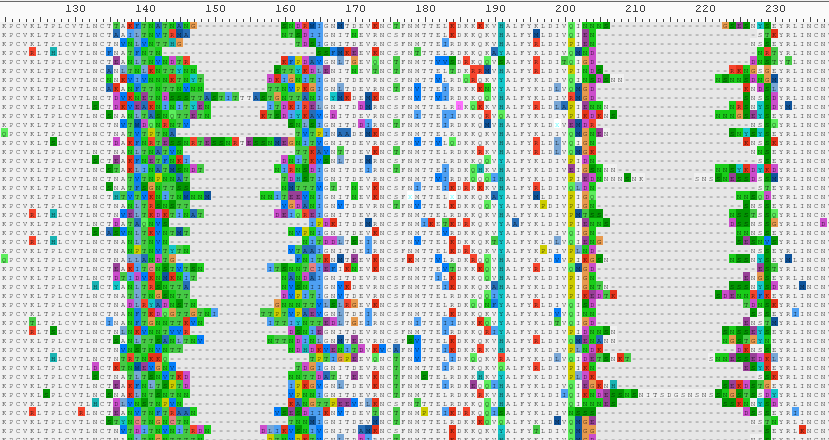
\includegraphics[height=3in,width=4in]{aliview.png}
\end{center}
Clearly, understanding the pattern of mutations and any relationships to treatment status for a particular site in the sequence is very difficult to do in this view with any precision.
\\
\newline
\noindent Other tools are geared towards specific analyses

\section{Project Plan}

Upcoming milestones, and subdivision of future work:
\begin{itemize}
  \item Add ability to choose from different color schemes (Graham?)
  	\begin{itemize}
	  \item Current color scheme follows that used by WebLogo. Discussion with the client suggests that other color schemes may also be desired.
	\end{itemize}
  \item Add ability to export charts (Wayne?)
  \item Reformatting site-selection area (Nick)
	\begin{itemize}
	  \item Data is long and skinny, number of sites desired from data is few (<10). Some zooming or focus/context option is needed, but ideal structure still TBD.
	  		Need to overcome issues in combining some subset of zooming, panning, brushing, and selecting.
	\end{itemize}
  \item Improved page formatting (all)
\end{itemize}

\end{document}

http://www.ncbi.nlm.nih.gov/pubmed/25095880